\chapter{Chi tiết Ontology Web Language}
\paragraph{Giới thiệu } - Như đã được đề cập trong phần cuối của chương trước, chức năng chính của OWL là một ngôn ngữ ontology cung cấp ngữ nghĩa cho Semantic Web. Trong nội dung chương này, chúng em sẽ giới thiệu về cú pháp, định dạng và chi tiết các đặc tính của ngôn ngữ Ontology Web. Phiên bản Ontology Web Language chúng em sử dụng là phiên bản 2 được tổ chức W3C khuyến khích sử dụng so với phiên bản OWL 1.1 .
\section{Khái quát về OWL 2 \cite{owl2}}
\subsection{Tổng quan}
\begin{figure}[ht!]
	\centering
	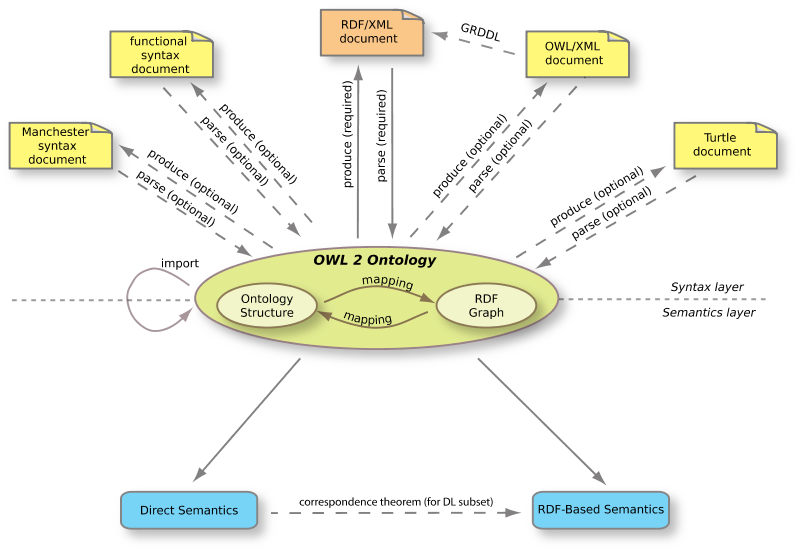
\includegraphics[width=120mm]{Figures/owl2structure.png}
	\caption{Cấu trúc của OWL 2\label{overflow}}
\end{figure}
Hình trên cho chúng ta cái nhìn tổng quan về các định dạng file, các loại cú pháp và cách khả năng serialization thành RDF Graph của Ontology. Như chúng ta thấy trong hình thì hình eclipse ở giữa thể hiện khái niệm trừu tượng của một ontology, có thể hiểu là một cấu trúc trừu tượng hay một đồ thi RDF. Chúng ta có thể dùng nhiều cú pháp để biểu diễn ontology và định dạng chúng dưới dạng file khác nhau (Syntex layer trong hình), các định dạng và cú pháp này hoàn toàn có thể chuyển đổi qua lại với nhau. Lớp ngữ nghĩa trong hình (semantic layer) cho thấy ngữ nghĩa được quy định theo 2 tiêu chuẩn kỹ thuật khác nhau là Direct Semantics và RDF-Based Semantics.
\\
Phần lớn những người phát triển Ontology bằng OWL2 sẽ chỉ cần 1 cú pháp (tương đương với 1 định dạng file) và một dạng biểu diễn ngữ nghĩa.
\subsection{Ontologies}
Bất kì ontology OWL2 nào đều có thể được định dạng như một đồ thị RDF. Mối quan hệ giữa 2 cách này được quy định bới cách tài liệu Mapping to RDF Graphs document [\href{http://www.w3.org/TR/owl2-overview/#ref-owl-2-rdf-mapping}{OWL 2 RDF Mapping}] \cite{mapping_rdf_graph}, trong tài liệu này định nghĩa rất rõ ràng một bảng map từ định dạng cấu trúc của ontology qua đồ thị RDF, và ngược lại. 
\subsection{Cú pháp}
Trong thực tế, một cú pháp cụ thể rất cần thiết để lưu trữ các OWL2 Ontologies và để trao đổi chúng giữa các công cụ và ứng dụng khác nhau. Cú pháp đầu tiên có khả năng hoán đổi là RDF/XML [\href{http://www.w3.org/TR/owl2-overview/#ref-rdf-syntax}{RDF Syntax}] \cite{rdfxml}. Ngoài RDF/XML có khả năng cung cấp khả năng tương tác giữ nhiều ứng dụng OWl2 khác nhau, các loại cú pháp khác đều có thể được sử dụng. Dưới đây là bảng so sánh và liệt kê các cú pháp.
\begin{table}[ht!]
\begin{tabular}{ |p{3cm}|p{4cm}|p{3cm}|p{4cm}|}
\hline
Tên cú pháp & Mô tả & Trạng thái & Mục đích sử dụng\\
\hline
RDF/XML & Mapping to RDF Graphs \cite{mapping_rdf_graph} \cite{rdfxml} & Bắt buộc & Hoán đổi được ( có thể viết và đọc được bằng nhiều phần mềm OWL2)
\\
\hline
OWL/XML & XML Serialization \cite{owlxml} & Tùy chọn & Xử lý dễ dàng hơn bằng công cụ XML.
\\
\hline
Functional Syntax & Structural Specification \cite{func_syntax} & Tùy chọn & Dễ đọc và hiểu được.
\\
\hline
Manchester Syntax & Manchester Syntax \cite{man_syntax} & Tùy chọn & Có ưu thế hơn để đọc/ghi DL Ontologies
\\
\hline
Turtle & Mapping to RDF Graphs \cite{mapping_rdf_graph} & Tùy chọn, không được công nhận chính thức & Có ưu thế để đọc/ghi RDF triples
\\
\hline
\end{tabular}
\caption{Bảng so sánh các cú pháp của OWL2\label{overflow}}
\end{table}
\subsection{Một số ví dụ của các syntax}
\subsubsection{Functional Syntax}
\begin{verbatim}
// Khai báo lớp
Declaration (Class (Animal)) l
Declaration (Class (Grass))) 
// Khai báo Object Property
Declaration (ObjectProperty (canEat))  
// Khai báo sub Class expression
SubClassOf (Cow Animal)  
// Khai báo sub Class Expression
SubClassOf (Cow ObjectSomeValueFrom(canEat Grass))  
\end{verbatim}
\subsubsection{RDF/XML Syntax}
\begin{verbatim}
T(Animal) rdf:type owl:Class
T(Grass) rdf:type owl:Class
T(canEat) rdf:type owl:ObjectProperty
T(Cow) rdfs:subClassOf T(Animal) 
T(Cow) rdfs:subClassOf T(_:x owl:someValuesFrom T(Grass))
\end{verbatim}
\subsubsection{OWL/XML Syntax}
\begin{verbatim}
<Declaration>
       <Class IRI="#Animal"/> // Khai báo lớp Animal
</Declaration>
<Declaration>
       <Class IRI="#Grass"/> // Khai báo lớp Grass
</Declaration>
<Declaration>
       <ObjectProperty IRI="#canEat"/> // Khai báo Object Property 
</Declaration>
<SubClassOf>
       <Class IRI="#Cow"/>
       <Class IRI="#Animal"/>  // Khai báo sub Class expression
</SubClassOf>
<SubClassOf>
       <Class IRI="#Cow"/>
<ObjectAllValuesFrom>
<ObjectProperty IRI="#canEat"/>  // Khai báo sub Class expression
       <Class IRI="#Grass"/>
</ObjectAllValuesFrom>
</SubClassOf>
\end{verbatim}
\subsubsection{Manchester Syntax}
\begin{verbatim}
Class: Cow 
    SubClassOf: Animal 
    SubClassOf: canEat some Grass
Class: Grass
ObjectProperty: canEat
\end{verbatim}
\section{Các đặc tính chi tiết của OWL2}
Ngôn ngữ Ontology Web Language 2 (hay OWL 2) đảm nhiệm chức năng thể hiện ngữ nghĩa cho Semantic Web như chúng ta đã thấy trong hình Semantic Web  Stack. OWL2 ontologies cung cấp các lớp (class), thuộc tính (property), cá thể (individual) và các giá trị dữ liệu (data value), tất cả chúng sẽ được biểu diễn bằng các tài liệu và cú pháp được đề cập ở trên, phần này sẽ đi vào giải thích các thành phần vừa nêu ra của một ontology được viết bằng ngôn ngữ OWL2 . Đây cũng chính là các thành phần cấu trúc mà thư viện OWLAPI \cite{owlapi} áp dụng để xây dựng nên bộ thư viện giúp người phát triển ứng dụng ontology tương tác dễ dàng hơn với các tài liệu ontology.
Đầu tiên chúng em xin được giới thiệu tới đối tượng lớn nhất trong quy định của ngôn ngữ OWL2.
\subsection{Ontologies}
\subsubsection{Ontology IRI và Version IRI}
Mỗi ontology đều có thế có\textit{một ontology IRI\cite{iri}} (Internationalized Resource Identifier), dùng để định danh cho ontology. Nếu một ontology có một ontology IRI, thì ontology này có thể có thêm một version IRI, dùng để xác định phiên bản cho ontology này. Version IRI có thể trùng hoặc không cần thiết phải trùng với ontology IRI. Một ontology không có ontology IRI thì không có version IRI.
Dưới đây là những quy ước chọn ontology IRIs và version IRIs trong OWL2. Những đặc điểm kỹ thuật này không cung cấp cơ chế nào để làm chúng phải được tuân theo trên toàn hệ thống web. Tuy nghiên, những công cụ hay ứng dụng OWl2 \textit{nên} sử dụng những quy ước này để dễ dàng tìm ra lỗi trong những ontology mà chúng xử lý.
\begin{itemize}
\item Nếu một ontology có một ontology IRI nhưng không có version IRI, thì \textit{không nên tồn tại} một ontology với trùng ontology IRI vừa đặt.
\item Nếu một ontology có một ontology IRI và một version IRI, thì \textit{không nên tồn tai} một ontology khác với trùng ontology IRI và version IRI vừa đặt.
\item Tất cả các cách kết hợp khác của ontology IRI và version IRI không cần đòi hỏi tính duy nhất (unique). Như vậy 2 ontologies khác nhau có thể không có ontology IRI và version IRI; tương tự, một ontology chưa một ontology IRI có thể cùng tồn tại cùng với một ontology khác có cùng ontology IRI vừa đặt \textbf{và} các version IRI của các ontologies này \textbf{phải} khác nhau.
\end{itemize}
Ontology IRI và các version IRI kết hợp với nhau giúp định danh một phiên bản cụ thể của của ontology từ một bộ chưa tất cả các phiên bản của một ontology cụ thể nào đó được định danh chung bằng ontology IRI. Trong mỗi bộ ontology như vậy, sẽ có chính xác một ontology được dùng nhưng một ontology hiện hành - khi dùng ontology IRI để truy vấn ontology mà không đề cập version IRI mặc định ontology co verison IRI hiện hành sẽ được trả về.

\subsubsection{Tài liệu Ontology}
Một OWL2 Ontology chỉ là một khái niệm trừu tượng chiếu theo định nghĩa trong các đặc tính cấu trúc của nó. Mỗi ontology gắn liền với một \textit{tài liệu ontology}
, chính là cách chúng ta thể hiện nội dụng ngữ nghĩa và lưu trữ chúng thành một dạng file nhất định ( như đã đề cập trong phần trên)










